\documentclass[../../../main.tex]{subfiles}

\begin{document}
\section{Electricitat i magnetisme}
\subsection{Anàlisi vectorial}
\begin{center}
\begin{tabular}{|c|c|}

    \hline
     & Fórmula (en coordenades rectangulars) \\
        \hline
    Gradient & $\displaystyle\grad f:=\Vec{\nabla}f=\frac{\partial f}{\partial x}\Vec{e}_x+\frac{\partial f}{\partial y}\Vec{e}_y+\frac{\partial f}{\partial z}\Vec{e}_z$ \\
        \hline
    Divergència & $\displaystyle\dive \Vec{A}:=\Vec{\nabla}\cdot\Vec{A}=\frac{\partial A_x}{\partial x}+\frac{\partial A_z}{\partial z}+\frac{\partial A_z}{\partial z}$\\
        \hline
    Rotacional & $\displaystyle\rot \Vec{A}:=\Vec{\nabla}\wedge\Vec{A}=\begin{vmatrix}
    \Vec{e}_x & \Vec{e}_y & \Vec{e}_z\\
    \frac{\partial}{\partial x} & \frac{\partial}{\partial y} & \frac{\partial}{\partial z}\\
    A_x & A_y & A_z\\
    \end{vmatrix}=\left(\frac{\partial A_z}{\partial z}-\frac{\partial A_y}{\partial y}\right)\Vec{e}_x+\left(\frac{\partial A_x}{\partial x}-\frac{\partial A_z}{\partial z}\right)\Vec{e}_y+\left(\frac{\partial A_y}{\partial y}-\frac{\partial A_x}{\partial x}\right)\Vec{e}_z$ \\
        \hline
   Laplaciana & $\displaystyle\nabla^2f:=\Vec{\nabla}\cdot\Vec{\nabla}f=\frac{\partial^2f}{\partial x^2}+\frac{\partial^2f}{\partial y^2}+\frac{\partial^2f}{\partial z^2}$ \\
        \hline
\end{tabular}
\end{center}
\begin{multicols}{2}
\subsection{Electroestàtica}
Quantització de la càrrega elèctrica: tota càrrega elèctrica és un múltiple de la càrrega fonamental.
$$Q=Ne$$
{on $e=1,602\times10^{-19}\;C$.}\newline
Equació de la continuïtat (conservació de la càrrega): $$\Vec{\nabla}\cdot\Vec{J}+\frac{\partial\rho}{\partial t}=0$$
{on $\rho$ és la densitat de càrrega i $\Vec{J}$ és la densitat de corrent.}\newline
Llei de Coulomb: $$\Vec{F}_{12}=k\frac{q_1q_2}{|\Vec{r}_{12}|^2}\Hat{r}_{12}$$
{on $k=\frac{1}{4\pi\epsilon_0}\approx8,99\times10^9$, $\Vec{r}_{12}=\Vec{r}_2-\Vec{r}_1$ i $\Hat{r}_{12}$ és el vector unitari que va de 1 a 2.}\newline
Principi de superposició: $$\Vec{F}_Q=kQ\sum_{i=1}^N\frac{q_i}{|\Vec{r}_i|^2}\Hat{r}_i$$
Camp elèctric: $$\Vec{E}=\frac{\Vec{F}}{q_2}=k\frac{q_1}{|\Vec{r}_{10}|^2}\Hat{r}_{10}$$
Principi de superposició de camps elèctrics:
\begin{itemize}
    \item Distribucions discretes de càrrega:
    $$\Vec{E}=k\sum_{i=1}^N\frac{q_i}{|\Vec{r}_{i0}|^2}\Hat{r}_{i0}$$
    \item Distribucions contínues de càrrega:
    $$\Vec{E}=\int d\Vec{E}=k\int\frac{dq}{|\Vec{r}|^2}\Hat{r}$$
    {on $dq=\rho dV$, $dq=\sigma dS$ o $dq=\lambda dl$ segons si es tracta de distribucions volumètriques, superficials o lineals, respectivament.}
\end{itemize}
Flux d'un camp vectorial $\Vec{A}$: 
\begin{gather*}
    d\Phi=\Vec{A}\cdot d\Vec{S}=AdS\cos\theta\\
    \Phi=\int d\Phi=\int_S\Vec{A}\cdot d\Vec{S}
\end{gather*}
Llei de Gau\ss:
$$\Phi=\oint_S\Vec{E}\cdot d\Vec{S}=\frac{Q_{\text{int}}}{\epsilon_0}$${on $\Phi$ és el flux elèctric.}\newline
Energia potencial electroestàtica:
\begin{gather*}
    dU=-\Vec{F}d\Vec{l}=-q_0\Vec{E}d\Vec{l}\\
    \int_a^bdU=\Delta U=U(b)-U(a)=-\int_a^bq_0\Vec{E}d\Vec{l}
\end{gather*}
Treball efectuat:
\begin{itemize}
    \item pel camp: $$W_{\text{camp}}=-\Delta U=U(a)-U(b)$$
    \item per forces externes: $$W_{\text{ext}}=\Delta U=U(b)-U(a)$$
\end{itemize}
Diferència de potencial:
\begin{gather*}
    dV:=\frac{dU}{q_0}=-\Vec{E}d\Vec{l}\\
    \Delta V=V(b)-V(a)=\frac{\Delta U}{q_0}=-\int_a^b\Vec{E}d\Vec{l}
\end{gather*}
Potencial creat per:
\begin{itemize}
    \item una càrrega puntual $q$: $$V(r)=\frac{kq}{r}$$
    \item una distribució discreta de càrregues: $$V=\sum_{i=1}^N\frac{kq_i}{r_{i0}}$$
    \item una distribució contínua de càrregues:
    $$V(b)-V(a)=\Delta V=-\int_a^b\Vec{E}d\Vec{l}$$
\end{itemize}
Energia electroestàtica:
\begin{itemize}
    \item Càrrega puntual $q$:$$U=q_0V=k\frac{qq_0}{r}$$
    \item Conjunt de càrregues puntuals: $$U=\frac{1}{2}\sum_{i,j}q_iV_j$$
    \item Distribució de càrrega:
    $$U=\frac{1}{2}\int\rho V d^3r$$
\end{itemize}
En un conductor en equilibri electroestàtic:
\begin{itemize}
    \item Tota la càrrega es troba en la superfície i el camp total dins el conductor és nul.
    \item El camp elèctric just a fora és per\-pen\-di\-cu\-lar a la superfície del conductor i val $\sigma/\epsilon_0$, on $\sigma$ és la densitat superficial de càrrega.
    \item El volum tancat pel conductor i la seva superfície són equipotencials.
\end{itemize}
Capacitat d'un condensador: $$C:=\frac{Q}{V}=\epsilon_0\frac{S}{d}$$ {on $S$ és la superfície de les plaques del condensador i $d$ és la distància de separació entre aquestes. $[C]=F$ (Farads).}\newline
Moment dipolar elèctric $\Vec{p}$: $$\Vec{p}=q\Vec{L}$$ {on $q$ és el valor absolut de les càrregues del dipol i $\Vec{L}$ és el vector desplaçament d'un pol a l'altre.}\newline
Energia potencial d'un dipol elèctric: $$U=-\Vec{p}\cdot\Vec{E}$$
Moment elèctric: $$\Vec{\tau}=\Vec{p}\wedge\Vec{E}$$ {on aquest moment tendeix a alinear el dipol amb el camp.}\newline
Constant dielèctrica $\kappa$: $$\epsilon=\kappa\epsilon_0$$
Energia emmagatzemada en un condensador: $$U=\frac{1}{2}CV^2=\frac{1}{2}QV=\frac{1}{2}\frac{Q^2}{C}$$
Densitat d'energia del camp elèctic $\eta_e$: $$\eta_e:=\frac{1}{2}\epsilon_0E^2$$
Associació de condensadors:
\begin{itemize}
    \item en sèrie:$$\frac{1}{C_{\text{eq}}}=\sum_i\frac{1}{C_i}$$
    \item en paral·lel: $$C_{\text{eq}}=\sum_iC_i$$ 
\end{itemize}
Intensitat de corrent: $$I:=\frac{dQ}{dt}$$
$$I=\int_S \Vec{J}\cdot d\Vec{S}$$ {on $\Vec{J}$ és la densitat de corrent.}\newline
Relació del corrent amb el moviment de càrregues:
$$I=\frac{\Delta Q}{\Delta t}=nqv_dS$$ {on $n$ és el nombre de portadors de càrrega $q$ per unitat de volum; $v_d$, la velocitat de deriva de les càrregues, i $S$, la secció del conductor.}
$$\Vec{J}=nq\Vec{v}_d$$
Llei d'Ohm microscòpica: $$\Vec{J}=\frac{ne^2\tau}{m_e}\Vec{E}=\sigma\Vec{E}$$ {on $\tau$ és el temps mitjà entre col·lisions de portadors; $m_e$, la massa de l'electró, i $\sigma$, la conductivitat. $[\sigma]=S/m$ (Siemens$/$metre).}\newline
Llei d'Ohm macroscòpica: $$I=\frac{V}{R}$$
Resistència i resistivitat: $$R=\rho\frac{l}{S}$$ {on $\rho=1/\sigma$ és la resistivitat del material de secció $S$ i longitud $l$.}\newline
Resistivitat en funció de la temperatura: $$\rho=\rho_0[1+\alpha(T-T_0)]$$ {on $\alpha$ és el coeficient de temperatura, $T_0$ és una temperatura fixada i $\rho_0$ és la resistivitat a $T_0$.}\newline
Potència elèctrica: $$P=\frac{dU}{dt}=I^2R=\frac{\Delta V^2}{R}$$
Associacions de resistències: 
\begin{itemize}
    \item en sèrie:$$R_{\text{eq}}=\sum_iR_i$$
    \item en paral·lel: $$\frac{1}{R_{\text{eq}}}=\sum_i\frac{1}{R_i}$$
\end{itemize}
Lleis de Kirchhoff:
\begin{enumerate}
    \item Regla dels nusos: en un nus del circuit on el corrent es pot dividir, la suma dels corrents que entren al nus ha de ser igual a la suma dels corrents que en surten. $$\sum_iI_i=0$$
    \item Regla de les malles: la suma de les diferències de potencial en una malla ha de ser igual a zero. $$\sum_iV_i=0$$
\end{enumerate}
Circuits RC ($\tau=RC$):
\begin{itemize}
    \item Càrrega d'un condensador:
    \begin{gather*}
        Q=Q_f(1-e^{-t/\tau})\\
        I=\frac{\xi}{R}e^{-t/\tau}
    \end{gather*}
    {on $\tau$ és la constant de temps del circuit; $Q_f$, la càrrega final del condensador, i $\xi$, la fem de la bateria.}
    \item Descàrrega d'un condensador:
    \begin{gather*}
        Q=Q_0e^{-t/\tau}\\
        I=I_0e^{-t/\tau}
    \end{gather*}
    {on $Q_0$ és la càrrega inicial del condensador, i $I_0$, la intensitat inicial que hi passa a través.}\textbf{}
\end{itemize}
\subsection{Magnetoestàtica}
Força exercida per un camp magnètic $\Vec{B}$ sobre una càrrega en moviment: $$\Vec{F}=q\Vec{v}\wedge\Vec{B}$$ {on $[B]=T$ (Tesla).}\newline
Força exercida per un camp magnètic $\Vec{B}$ sobre un element de corrent $Id\Vec{l}$: $$d\Vec{F}=Id\Vec{l}\wedge\Vec{B}$$
La força magnètica no realitza treball sobre la partícula.\newline
Trajectòria de la partícula:
\begin{itemize}
    \item $\Vec{v}\perp\Vec{B}\implies$ òrbita circular. Radi de l'òrbita:$$r=\frac{mv_\perp}{qB}$$
    \item $\Vec{v}\not\perp\Vec{B}\implies\Vec{v}=\Vec{v}_\perp+\Vec{v}_\parallel\implies$ trajectòria helicoïdal.
\end{itemize}
Força de Lorentz (força electromagnètica): $$\Vec{F}=q(\Vec{E}+\Vec{v}\wedge\Vec{B})$$
Moment dipolar magnètic $\Vec{\mu}$: $$\Vec{\mu}=NI\Vec{S}$$
Moment magnètic: $$\Vec{\tau}=\Vec{\mu}\wedge\Vec{B}$$ 
Treball per rotar una espira: $$U=-\Vec{\mu}\cdot\Vec{B}$$
Força magnètica sobre un dipol (que no gira sobre si mateix): $$F_{\text{ext}}=\Vec{\nabla}(\Vec{\mu}\cdot\Vec{B})$$
Efecte Hall:\newline
\begin{minipage}{\linewidth}
    \centering
    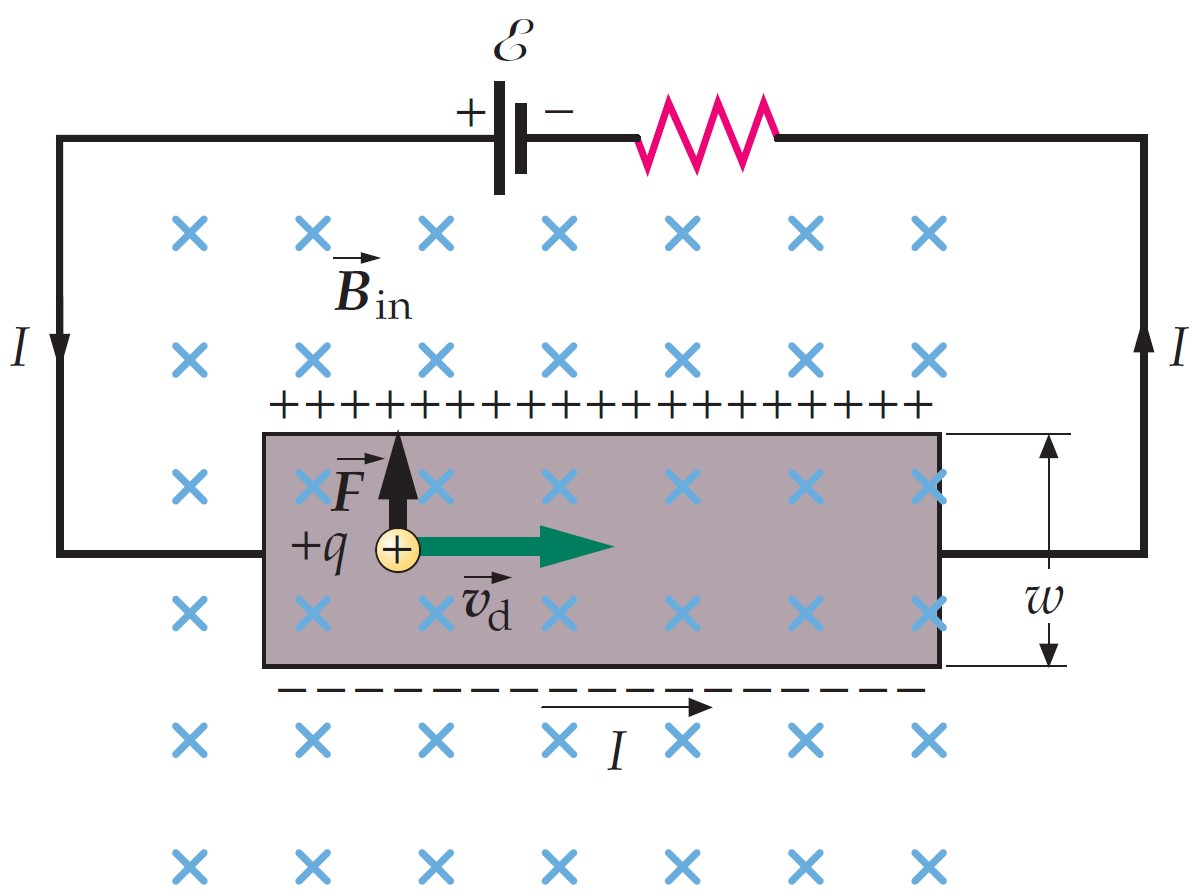
\includegraphics[width=\linewidth]{Physics/1st/Electricity_and_magnetism/Images/hall+.jpg}
    \captionof{figure}{Efecte Hall quan circulen càrregues positives pel circuit.}
\end{minipage}
\begin{minipage}{\linewidth}
    \centering
    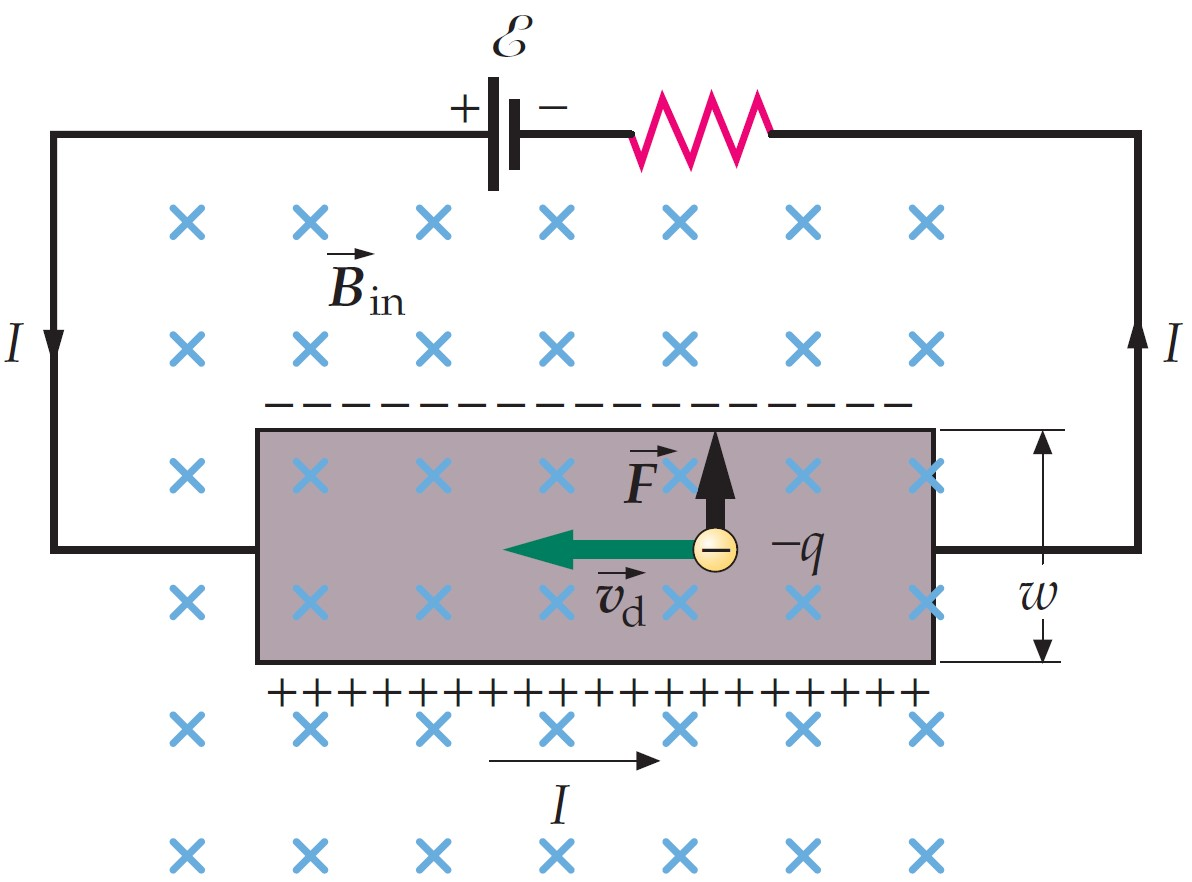
\includegraphics[width=\linewidth]{Physics/1st/Electricity_and_magnetism/Images/hall-.jpg} 
    \captionof{figure}{Efecte Hall quan circulen càrregues negatives pel circuit}   
\end{minipage}
S'usa per:
\begin{itemize}
    \item determinar el nombre de portadors de càrrega $n$: $$n=\frac{IB}{qdV_H}$$ {on $d$ és l'amplada del material conductor i $V_H$ és el voltatge de Hall, és a dir, la di\-fe\-rèn\-ci\-a de potencial entre els extrems superior i inferior del material conductor.}
    \item mesurar la intensitat del camp mag\-nè\-tic: $$V_H=\frac{I}{nqd}B$$
\end{itemize}
Camp magnètic creat per una càrrega puntual en moviment: $$\Vec{B}=\frac{\mu_0}{4\pi}\frac{q\Vec{v}\wedge\Hat{r}}{|\Vec{r}|^2}$$ {on $\Hat{r}=\Vec{r}/|\Vec{r}|$ és el vector unitari en la direcció de $\Vec{r}$.}\newline
Camp magnètic creat per un element de corrent (Llei de Biot-Savart): $$d\Vec{B}=\frac{\mu_0}{4\pi}\frac{Id\Vec{l}\wedge\Vec{r}}{|\Vec{r}|^3}$$
Camp magnètic $\Vec{B}$ creat per:
\begin{itemize}
    \item una espira circular de radi $R$:
    \begin{itemize}
        \item En un punt qualsevol del seu eix a distància $x$ del seu centre: $$\Vec{B}=\frac{\mu_0}{2}\frac{R^2I}{(x^2+R^2)^{3/2}}\Vec{e}_x$$
        \item En el seu centre: $$\Vec{B}=\frac{\mu_0I}{2R}\Vec{e}_x$$
    \end{itemize}
    \item un solenoide de radi $R$, longitud $L$ i densitat d'espires $n=N/L$ situat entre $x=-a$ i $x=b$:
    \begin{itemize}
        \item En un punt qualsevol del seu eix a distància $x$ del seu centre:
        \begin{footnotesize}
            \begin{multline*} \Vec{B}=\frac{\mu_0}{2}\frac{nI}{a+b}\left(\frac{b-x}{\sqrt{(b-x)^2+R^2}}+\right.\\\left.+\frac{a+x}{\sqrt{(a+x)^2+R^2}}\right)\Vec{e}_x
            \end{multline*}
        \end{footnotesize}
        \item En el seu centre ($a,b>>R$): $$\Vec{B}=\mu_0 nI\Vec{e}_x$$
    \end{itemize}
    \item un fil a un punt $P$ tal que l'angle entre l'eix vertical i els vectors directors de $P$ als extrems del fil són $\theta_1$ i $\theta_2$:\newline
    \begin{minipage}{\linewidth}
        \centering
        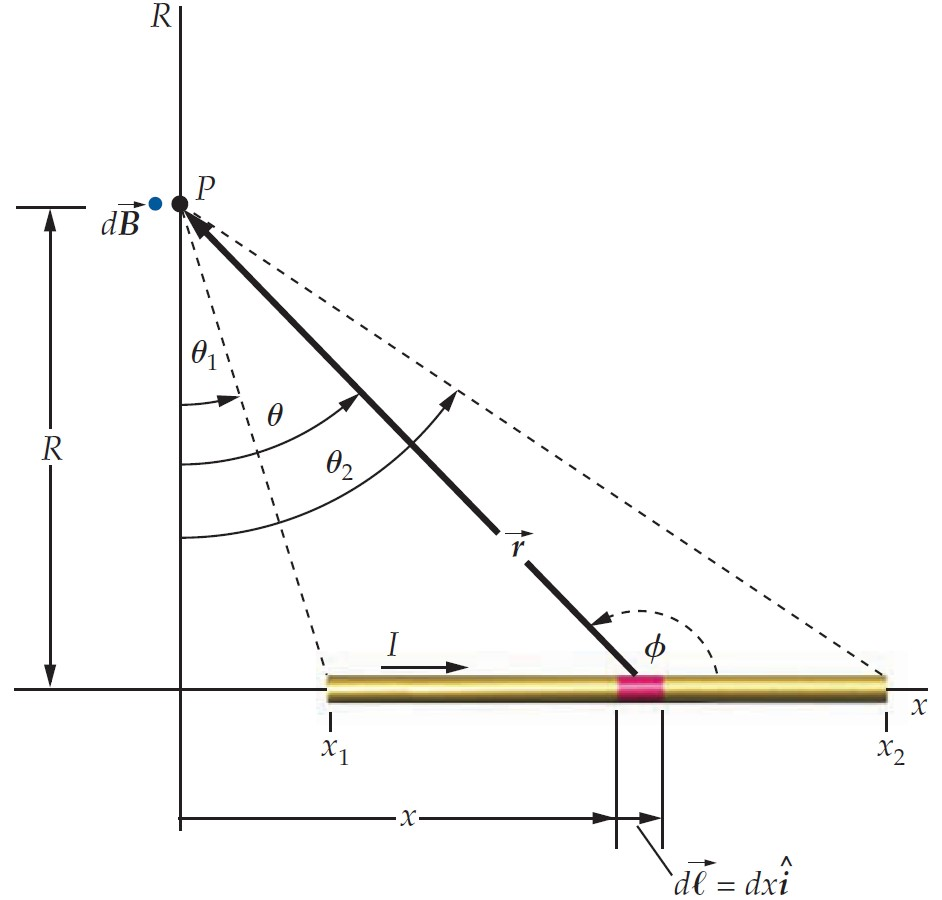
\includegraphics[width=7cm]{Physics/1st/Electricity_and_magnetism/Images/fil.jpg} 
    \end{minipage}
    \begin{itemize}
        \item fil finit: $$B=\frac{\mu_0I}{4\pi R}(\sin\theta_1+\sin\theta_2)$$
        \item fil infinit ($\theta_1\to-\pi/2,\theta_2\to\pi/2$): $$B=\frac{\mu_0I}{2\pi R}$$
    \end{itemize}
\end{itemize}
Força per unitat de longitud entre dos cables paral·lels transportant intensitats $I_1$ i $I_2$ res\-pec\-ti\-va\-ment, separats per una distància $d$: $$\frac{F}{l}=\frac{\mu_0}{2\pi}\frac{I_1I_2}{d}$$
Llei de Gau\ss\ pel magnetisme: $$\oint\Vec{B}\cdot d\Vec{S}=0$$
Llei d'Ampère: $$\oint\Vec{B}\cdot d\Vec{l}=\mu_0I_{\text{int}}$$
Camp magnètic creat per un anell toroïdal de $N$ espires i de radi interior $a$ i exterior $b$: $$B=\left\{
    \begin{array}{ccc}
    0 & \text{si} & r<a\text{ o }r>b \\
    \displaystyle\frac{\mu_0NI}{2\pi r} & \text{si} & a<r<b
    \end{array}\right.$$
Relació entre el moment angular orbital $\Vec{L}$ i el moment magnètic $\Vec{\mu}$: $$\Vec{\mu}=\frac{q}{2m}\Vec{L}$$
El moment angular està quantitzat.\newline
Magnetó de Bohr: $$\mu_B=\frac{e\hslash}{2m_e}\approx9,274\times10^{-24}\;J/T$$
Moments magnètics causats pel moment angular i spin d'un electró:
$$\Vec{\mu}_L=-\mu_B\frac{\Vec{L}}{\hslash}\quad\qquad\Vec{\mu}_S=-2\mu_B\frac{\Vec{S}}{\hslash}$$ {on $\Vec{S}$ és l'spin de l'electró.}\newline
Moment angular total: $$\Vec{J}=\Vec{L}+\Vec{S}$$
Imantació: $$\Vec{M}=\frac{d\Vec{\mu}}{dV}=\frac{di}{dl}$$ {on $\Vec{M}$ és el moment dipolar magnètic net per unitat de volum.}
$$\Vec{M}=\frac{1}{V}\sum_i\Vec{\mu}_i$$
Imantació de saturació: $$M_s=n\cdot\Vec{\mu}$$ {on $n$ és el nombre d'àtoms per unitat de volum.}\newline
La imantació de saturació es produeix quan tots els àtoms tenen els seus moments magnètics alineats.\newline
Camp generat:
$$\Vec{B}_{\text{gen}}=\mu_0\Vec{M}$$
Intensitat del camp magnètic: \begin{gather*}
\Vec{H}=\frac{\Vec{B}}{\mu_0}\\
\Vec{M}=\chi_m\Vec{H}
\end{gather*}
{on $\chi_m$ és la susceptibilitat magnètica. Aquesta no té dimensions i representa el grau de magnetització del material en resposta a un camp magnètic aplicat.}\newline
Camp aplicat i camp generat: Considerem un cil·lindre conductor pel qual circula una intensitat de corrent sotmès dins d'un solenoide, pel qual també circula una intensitat de corrent. El camp total del cil·lindre serà la suma dels camps generat (per aquest mateix) i aplicat (el generat pel solenoide): $$\Vec{B}_T=\Vec{B}_{\text{apl}}+\Vec{B}_{\text{gen}}=\mu_0\Vec{H}(1+\chi_m)$$
Tipus de materials:
\begin{itemize}
    \item Ferromagnètics (Fe, Ni, Co, $\ldots$): $\chi_m\in(10^2,10^5)\rightarrow$ Atracció forta\newline Els materials ferromagnètics presenten un fenomen anomenat \textit{exchange interaction}. L'\textit{exchange interaction} és un efecte descrit per la mecànica quàntica que ocorre entre electrons d’un mateix àtom aparellats o de diferents àtoms quan superposen les seves funcions d’ona (quan estan molt a prop). Quan això passa, poden alinear-se entre ells de forma que es minimitza l’energia del conjunt. Això genera els anomenats dominis magnètics, que són regions microscòpiques del material on els moments magnètics estan alineats.\newline
    Cicle d'histèresi:\newline
    \begin{minipage}{\linewidth}
        \centering
        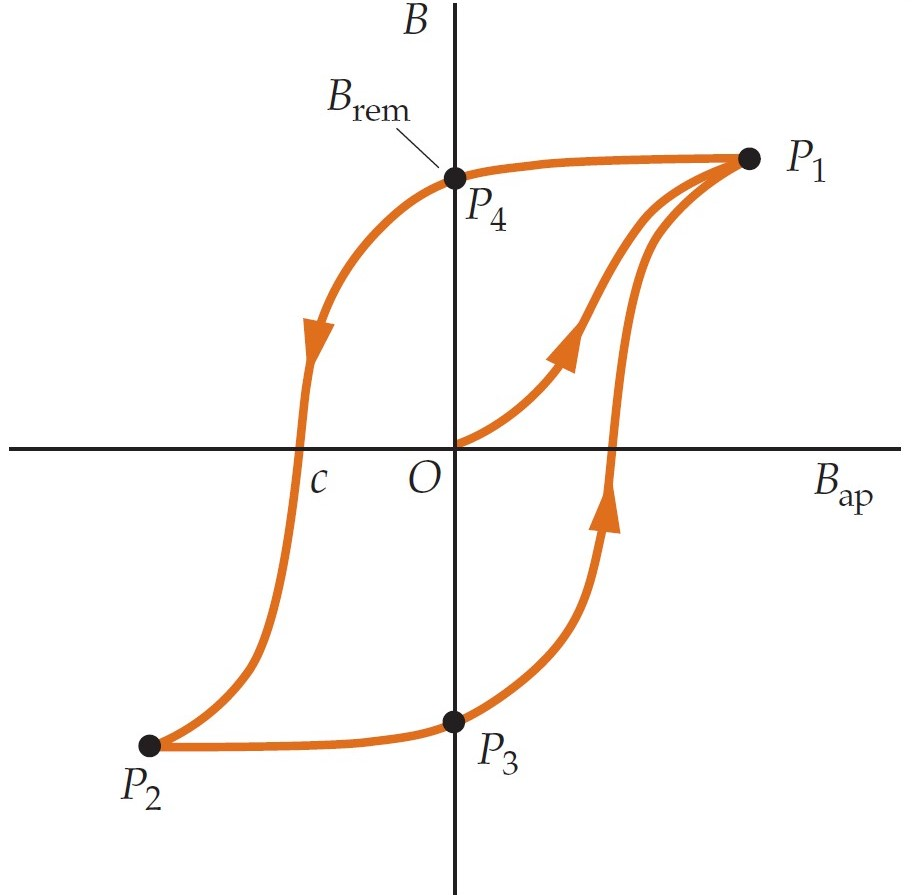
\includegraphics[width=7cm]{Physics/1st/Electricity_and_magnetism/Images/hist.jpg}
        \captionof{figure}{Cicle d'histèresi (procés d'i\-man\-ta\-ció d'un material ferromagnètic). Si augmentem el camp aplicant $B_\text{ap}$ sobre el material, el camp del material també anirà augmentant (línia del mig), i el seu ritme anirà disminuint perquè s’apropa al límit (imantació de saturació). Si ara comencem a reduir la intensitat del camp aplicat, el camp del material disminuirà, però sense seguir el mateix camí d’abans, sinó que disminuirà a un ritme més lent del què pujava. Com a conseqüència, quan $B_\text{ap}=0$, el camp del material encara no s’haurà anul·lat del tot, sinó que quedarà un camp $B_\text{rem}$ anomenat camp romanent. Si ara continuem el cicle invertint la direcció de $B_\text{ap}$, la intensitat del camp del material continuarà disminuint, i a un cert punt $B_\text{c}$ (camp coercitiu) el camp magnètic del material s’anul·larà del tot. Des\-prés es pot continuar el cicle fins que el camp del material arriba a un altre màxim (però ara en l’altra direcció) i així es repeteix el cicle. L'àrea tancada dins la corba del cicle d'histèresi depèn del tipus de material. Quan un material és dur vol dir que té un camp romanent intens i, per tant, aquesta àrea serà major. Si el material és tou, aquest gairebé no presenta memòria pel fet d’haver estat imantat i, per tant, torna gairebé pel mateix camí. L'àrea tancada dins la corba és proporcional a l'energia dissipada en els processos de magnetització i desmagnetització.}
    \end{minipage}
    \item Paramagnètics (Al, Mg, O$_2$, $\ldots$): $\chi_m\in(10^{-5},10^{-2})\rightarrow$ Atracció feble\newline Si hi ha camp, els moments magnètics comencen a alinear-se formant un camp. Ara bé, com que les in\-te\-rac\-cions atòmiques no són gaire fortes, els àtoms són susceptibles a l’agitació tèrmica, la qual indueix un moviment aleatori en els àtoms. Això provoca que l'energia tèrmica d'un material paramagnètic sigui molt més gran que l’energia magnètica.\newline La temperatura de Curie és una temperatura a partir de la qual un material pot passar de ser paramagnètic a ser ferromagnètic. Per sota d’aquesta temperatura el material és ferromagnètic i per sobre d'aquesta, paramagnètic.\newline
    En camps febles $\rightarrow$ llei de Curie: $$M=\frac{1}{3}\frac{\mu B_\text{ap}}{k_B T}M_s$$ {és a dir, la imantació creix linealment en funció de la imantació de saturació.}
    \item Diamagnètics (Bi, Ag, Hg, $\ldots$): $\chi_m\in(-10^{-6},-10^{-4})$ $\rightarrow$ Repulsió feble\newline El diamagnetisme es produeix per la presència d’un camp magnètic, que provoca que el moment magnètic orbital generi un camp en sentit contrari. Aquest fenomen passa en tots els materials, però com que els moments magnètics induïts són molt petits, els fenòmens de paramagnetisme i ferromagnetisme el superen.
\end{itemize}
Permeabilitat magnètica: $$\mu=(1+\chi_m)\mu_0=\kappa_m\mu_0$$
Flux magnètic: $$\Phi_B=\int_S\Vec{B}\cdot d\Vec{S}$$
Si tenim $N$ espires i $B$ és constant: $$\Phi=NBS\cos\theta$$
Llei de Faraday: $$\xi=\oint\Vec{E}\cdot d\Vec{l}=-\frac{d\Phi_B}{dt}$$ {on $\xi$ és la força electromotriu induïda.}\newline
Llei de Lenz: La fem i el corrent induït tenen una direcció i sentit que tendeixen a oposar-se a la variació que les produeix.\newline
Inducció d'un camp elèctric $E$ a partir d'una espira de radi $r$: $$E=-\frac{r}{2}\frac{dB}{dt}$$
Inducció electromagnètica: $$\frac{d\Phi_B}{dt}=\left(\frac{\partial\Phi}{\partial t}\right)_{v=0}+\left(\frac{\partial\Phi}{\partial t}\right)_{B=cte}$$
Generació de corrent altern: 
\begin{gather*}
    V=NBS\omega\sin\omega t=V_0\sin\omega t\\
    I=\frac{V_0}{R}\sin\omega t
\end{gather*}
{Té l’inconvenient que no s’aprofita sempre l’energia, ja que hi ha moments en què la força electromotriu s’anul·la. Per evitar-ho, es fa servir corrent trifàsic: tres espires amb un angle de desfasament de $120^\circ$ entre si.}\newline
Corrents de Foucault: Corrents circulars produïdes en un tros de metall per fluxos magnètics variables. Aquests corrents indueixen una força magnètica que s’oposa al moviment.\newline
Autoinductància $L$:
$$\Phi_B=LI$$ {on $[L]=H$ (Henry).}\newline
Autoinductància per una bobina de longitud $l$, secció $S$ i densitat d'espires $n$: $$L=\mu_0n^2Sl$$
Fem induïda fent variar el corrent elèctric: $$\xi=-L\frac{dI}{dt}$$
Diferència de potencial entre els extrems d'un inductor: $$\Delta V=-L\frac{dI}{dt}-Ir$$ {on $r$ és la resistència interna de l'inductor.}\newline
Inductància mútua:
\begin{gather*}
    \Phi_{m1}=L_1I_1+M_{12}I_2\\
    \Phi_{m2}=L_2I_2+M_{21}I_1
\end{gather*}
{on $M_{12}=M_{21}=M$ és el coeficient d'inducció mútua ($[M]=H$).}\newline
Circuits RL ($\tau=L/R$):
\begin{itemize}
    \item Connexió amb la bateria: $$I=\frac{\xi}{R}(1-e^{-t/\tau})$$
    \item Desconnexió de la bateria: $$I=\frac{\xi}{R}e^{-t/\tau}$$
\end{itemize}
Energia magnètica emmagatzemada en un inductor: $$U_m=\frac{1}{2}LI^2$$
Densitat d'energia magnètica $\eta_m$: $$\eta_m=\frac{1}{2}\frac{B^2}{\mu_0}$$
Velocitat d'ones electromagnètiques al buit: $$v=\frac{1}{\sqrt{\epsilon_0\mu_0}}=c$$
\end{multicols}
\begin{table}[ht]
    \centering
    \renewcommand{\arraystretch}{3}
    \begin{tabular}{|c|c|c|}
    \hline
    \bfseries Llei & \bfseries Forma diferencial &\bfseries Forma integral \\
         \hline
    de Gau\ss & $\displaystyle \Vec{\nabla}\cdot\Vec{E}=\frac{\rho}{\epsilon_0}$ & $\displaystyle \oint_S\Vec{E}\cdot d\Vec{S}=\frac{Q_{\text{int}}}{\epsilon_0}$ \\
     \hline
    de Gau\ss\ (magnetisme) & $\displaystyle \Vec{\nabla}\cdot\Vec{B}=0$ & $\displaystyle \oint_S\Vec{B}\cdot d\Vec{S}=0$\\
     \hline
    de Faraday-Lenz & $\displaystyle \Vec{\nabla}\wedge\Vec{E}=-\frac{\partial\Vec{B}}{\partial t}$ & $\displaystyle \oint_C\Vec{E}\cdot d\Vec{l}=-\frac{d}{dt}\int_S\Vec{B}\cdot d\Vec{S}$ \\
          \hline
    d'Ampère-Maxwell & $\displaystyle \Vec{\nabla}\wedge\Vec{B}=\mu_0\Vec{J}+\mu_0\epsilon_0\frac{\partial\Vec{E}}{\partial t}$ & $\displaystyle \oint_C\Vec{B}\cdot d\Vec{l}=\mu_0 I+\mu_0\epsilon_0\frac{d}{dt}\int_S\Vec{E}\cdot d\Vec{S}$\\
          \hline
\end{tabular}
    \captionof{figure}{Equacions de Maxwell.}
    \label{tab:my_label}
\end{table}
\end{document}